\documentclass[12pt,twoside]{article}
\usepackage{light}
\usepackage{subfigure}
\usepackage{graphicx}
\hidesolutions
\showsolutions

%Solutions are currently incorrect
\begin{document}

\begin{problem}{10}
\bparts
\ppart{2} Does the above graph have a Hamiltonian path?

\ppart{2} Does the above graph have a Eulerian path?

\ppart{6} Consider the complete graph on $n$ vertices $K_n$ for odd $n \geq 3$.  Prove that we cannot find a series of Hamiltonian paths in $K_n$ that together cover all the edges of $K_n$.  

\eparts
\end{problem}

%%%%%%%%%%%%%%%%%%%%%%%%%%%%%%%%%%%%%%%%%%%%%%%%%%%%%

%\newpage

%%%%%%%%%%%%%%%%%%%%%%%%%%%%%%%%%%%%%%%%%%%%%%%%%%%%%


\begin{problem}{10}
\bparts
\ppart{3}  Find $7^{100}$ mod $13$.

\ppart{3} Find the inverse of $33$ mod $121$ or prove that no such inverse exists.

\ppart{4} Prove that for any non-zero integers $a, b, c, d$, if $a - c \mid ab + cd$, then $a - c \mid ad + bc$.

\eparts
\end{problem}

%%%%%%%%%%%%%%%%%%%%%%%%%%%%%%%%%%%%%%%%%%%%%%%%%%%%%

%\newpage

%%%%%%%%%%%%%%%%%%%%%%%%%%%%%%%%%%%%%%%%%%%%%%%%%%%%%


\begin{problem}{10}
\bparts
\ppart{}
\eparts
\end{problem}

\begin{problem}{16} 
A portion of a computer program consists of a sequence of calculations
where the results are stored in variables, like this:
\[
\begin{array}{rrrcl}
&& \text{Inputs:} &  & x, y \\
\text{Step } 1. & \hspace{0.5in} & a & = & x - 24 \\
2. && b & = & x * a \\
3. && c & = & 3 \\
4. && d & = & y - c \\
5. && e & = & y ** c \\
6. && f & = & e + 1  \\
&& \text{Outputs:} & & b, d, e
\end{array}
\]
A computer can perform such calculations most quickly if the value of
each variable is stored in a \emph{register}, a chunk of very fast
memory inside the microprocessor.  Programming language compilers face
the problem of assigning each variable in a program to a register.
Computers usually have few registers, however, so they must be used
wisely and reused often.  This is called the \emph{register
  allocation} problem.

In the example above, variables $x$ and $y$ must be assigned different
registers, because they hold distinct input values.  Furthermore, $c$
and $d$ must be assigned different registers; if they used the same
one, then the value of $c$ would be overwritten in the fourth step and
we'd get the wrong answer in the fifth step.  On the other hand,
variables $b$ and $d$ may use the same register; we no longer need $b$ and can overwrite the register that holds its
value.  Assume that the computer carries out each step in the order
listed and that each step is completed before the next is begun.

\bparts

\ppart{6} Recast the register allocation problem as a question
about graph coloring.  What do the vertices correspond to?  Construct
the graph corresponding to the example above.

\solution{
There is one vertex for each variable.  An edge between two vertices
indicates that the values of the variables must be stored in different
registers.  We can tell when two variables must be stored in different
registers as follows: classify each appearance of a variable in the
program as either an \emph{assignment} or a \emph{use}.  An appearance
is an \emph{assignment} when the variable is on the left side of an
equation or on the ``Inputs'' line.  An appearance of a variable is a
\emph{use} if the variable is on the right side of
an equation or on the ``Outputs'' line.  The \emph{lifetime} of a variable is the segment of code
extending from the initial assignment of the variable until the last
use.  There is an edge between two variables iff their lifetimes
overlap.

  We are also assuming that all variables are relevant to the Outputs,
  where a variable is \emph{relevant} iff it
  is an Output or is used in an assignment to a relevant variable.
  This is a recursive---not a circular---definition of relevant
  variable!

  Likewise, we assume that all variables are \emph{dependent} on the Inputs, where a variable is
  dependent on the Inputs iff it is an Input or appears in the left
  hand side of an assignment whose right hand side contains a
  dependent variable.
}

\ppart{5} How many registers
do you need?

\solution{
Four registers are needed.

One possible assignment of variables to registers is indicated in the
figure above.  In general, coloring a graph using the minimum number
of colors is quite difficult; no efficient procedure is known.
However, the register allocation problem always leads to an
\term{interval graph}, and optimal colorings for interval graphs are
always easy to find.  This makes it easy for compilers to allocate a
minimum number of registers.
}

\eparts
\end{problem}



\begin{problem}
A \emph{multiple binary-tree network} has $n$ inputs and $n$ outputs, where $n$ is
a power of 2.  Each input is connected to the root of a binary tree with
$n/2$ leaves and with edges pointing away from the root.  Likewise, each
output is connected to the root of a binary tree with $n/2$ leaves and
with edges pointing toward the root.

Two edges point from each leaf of an input tree, and each of these edges
points to a leaf of an output tree.  The matching of leaf edges is
arranged so that for every input and output tree, there is an edge from a
leaf of the input tree to a leaf of the output tree, and every output tree
leaf has exactly two edges pointing to it.

\bparts
\ppart Draw such a multiple binary-tree net for $n=4$.

\solution{
\begin{figure}[h]
%\graphic{binnet}
\centering
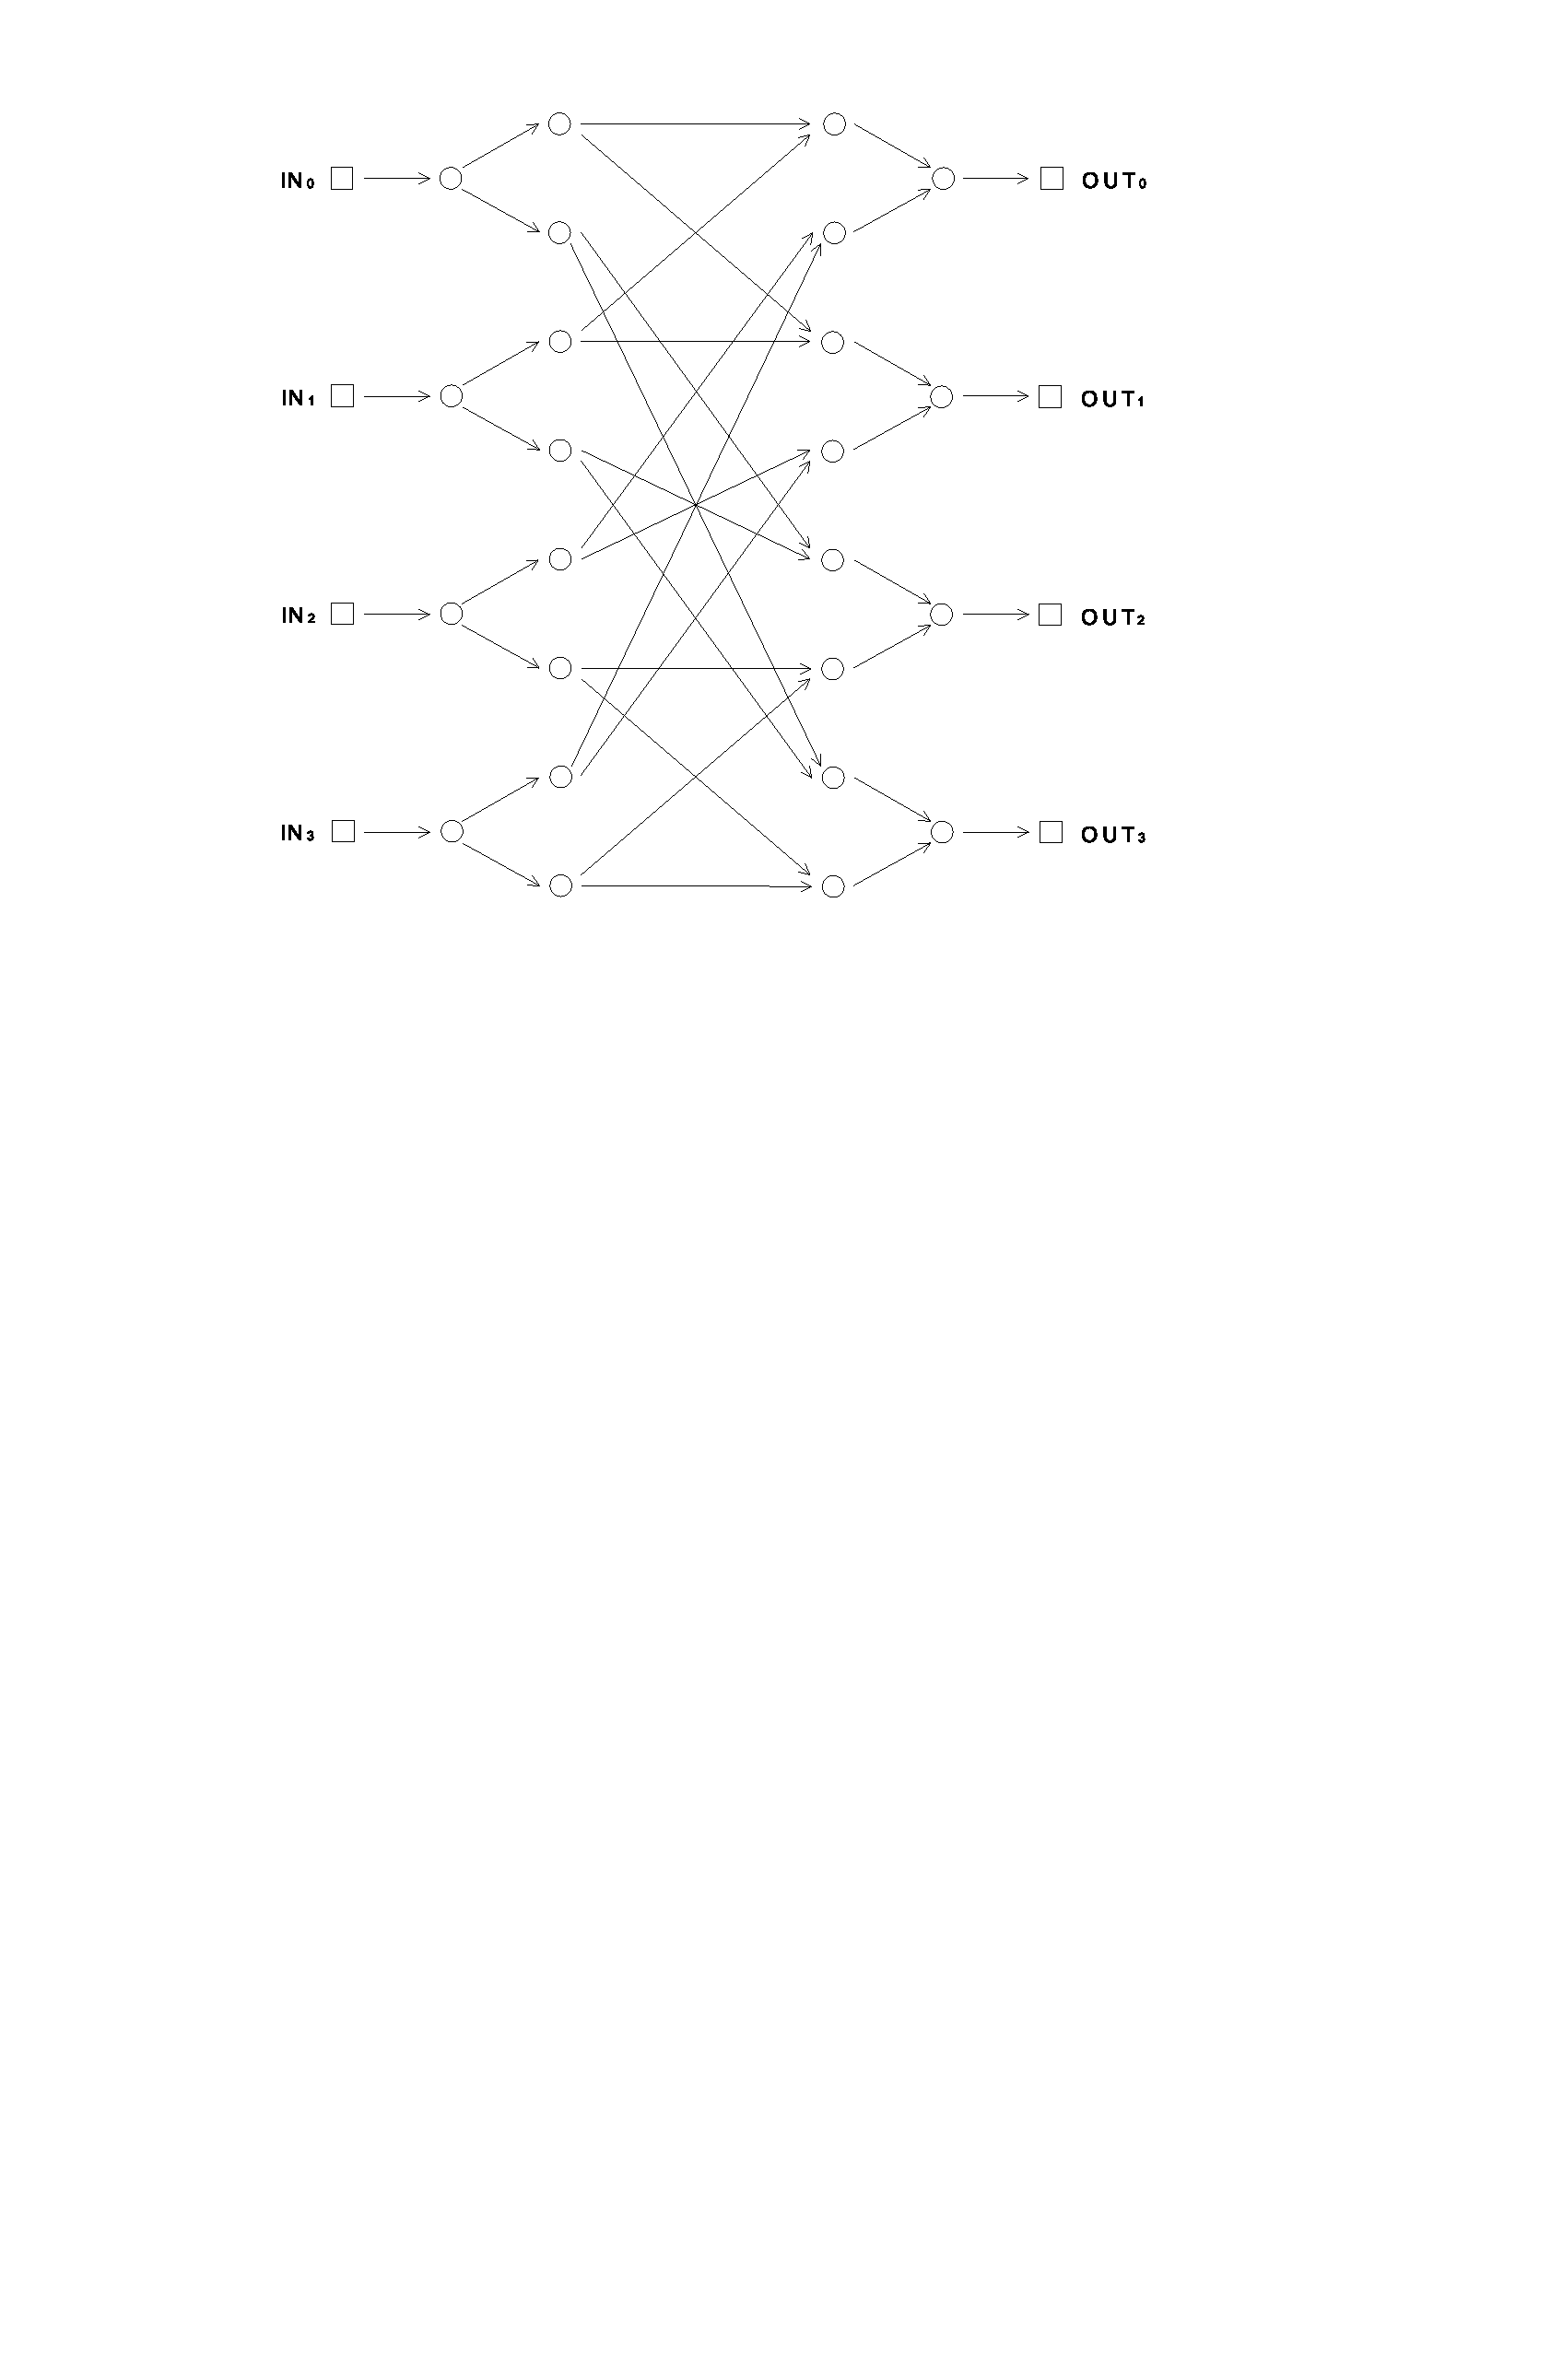
\includegraphics[scale=1]{binnet}
\end{figure}
}

\ppart Fill in the table, and explain your entries.

{\large
\[
\begin{array}{c|c|c|c}
\text{\# switches} &
\text{switch size} &
\text{diameter} &
\text{max congestion} \\ \hline
&&&\\ \hline
\end{array}
\]
}

\begin{solution}
{\large
\[
\begin{array}{c|c|c|c}
\text{\# switches} &
\text{switch size} &
\text{diameter} &
\text{max congestion} \\ \hline
2n(n-1)& 1 \times 2, 2 \times 1 & 1+ 2\log n & 1\\ \hline
\end{array}
\]
}

\iffalse
\begin{align*}
\text{\# switches } & = 2n(n-1)\\
\text{switch size} & = 1 \times 2, 2 \times 1\\
\text{diameter} & =  1+ 2\log n\\
\text{max congestion} & =1
\end{align*}
\fi

These formulas were gotten as follows: a binary tree with $n/2$ leaves has
$n-1$ nodes (switches), and there are $2n$ trees.

Each node of an input tree has one edge in and two out; the opposite
for nodes of output trees.

The distance from any input to any output is 1 from input to tree root,
$(\log n)-1$ from root to leaf, 1 from input leaf to output leaf, $(\log
n)-1$ from output leaf to output root, and 1 to output, for a total of $1+
2\log n$.

The path from any input to any output is unique, and paths from two inputs
to different outputs don't overlap, so at most one packet goes through any
switch.
\end{solution}

\eparts

\end{problem}


\end{document}
